\documentclass[../main.tex]{subfiles}

\begin{document}
\section{10.4 - Optimal Control of Pitch/Travel and Elevation with Feedback}
In the previous labs the elevation has been disregarded, and assumed to be zero. In this lab, elevation is not disregarded, and the group had to calculate an optimal trajectory for the elevation as well. 

\subsection{The continuous model}
\textit{Answer 10.4.1.1}
The equation for elevation has been given in the problem description as
\begin{equation}\label{eq:lab4_elevation}
	\ddot{e} + K_3K_{ed}\dot{e} + K_3K_{ep}e = K_3K_{ep}e_c
\end{equation}
where $ e_c $ is the elevation setpoint.

Expanding the system defined in \cref{eq:lab2_cont_ss} to include \cref{eq:lab4_elevation}, gives a new system that includes the elevation:

\begin{equation}\label{eq:lab4_cont_ss}
	\underbrace{\begin{bmatrix}
			\dot \lambda \\
			\dot r \\
			\dot p \\
			\ddot p \\
			\dot e \\
			\ddot e \\
	\end{bmatrix}}_{\bm{\dot x}} = 
	\underbrace{
		\begin{bmatrix}
			0 & 1 & 0 & 0 & 0 & 0\\
			0 & 0 & -K_2 & 0 & 0 & 0\\
			0 & 0 & 0 & 1 & 0 & 0\\
			0 & 0 & -K_1 K_{pp} &  -K_1 K_{pd} & 0 & 0\\
			0 & 0 & 0 & 0 & 0 & 1 \\
			0 & 0 & 0 & 0 & -K_3K_{ep} & -K_3K_{ed} \\
		\end{bmatrix}
	}_{\bm A_c}
	\underbrace{
		\begin{bmatrix}
			\lambda \\ r \\ p \\ \dot{p} \\ e \\ \dot{e}
		\end{bmatrix}
	}_{\bm x}
	+
	\underbrace{
		\begin{bmatrix}
			0 & 0 \\
			0 & 0\\
			0 & 0\\
			K_1 K_{pp} & 0\\
			0 & 0 \\
			0 & K_3K_{ep} \\
		\end{bmatrix}
	}_{\bm B_c} 
	\underbrace{
		\begin{bmatrix}
			p_c \\
			e_c \\
		\end{bmatrix}
	}_{\bm u}
\end{equation}

\subsection{The discretized model}
\textit{Answer 10.4.1.2}
Discretizing the continuous system defined in \cref{eq:lab4_cont_ss} was done using the forward Euler method (see \cref{sec:lab2_disc} for more information about this method).

The resulting dicretized system became: 
\begin{equation}\label{eq:lab4_disc_ss}
	\bm A_d = \begin{bmatrix}
		1 & T & 0 & 0 & 0 & 0\\
		0 & 1 & -TK_2 & 0 & 0 & 0\\
		0 & 0 & 1 & T & 0 & 0\\
		0 & 0 & -T K_1 K_{pp} &  1 - T K_1 K_{pd} & 0 & 0\\
		0 & 0 & 0 & 0 & 1 & T \\
		0 & 0 & 0 & 0 & -T K_3 K_{ep} & 1 - TK_3K_{ed} \\
	\end{bmatrix}, \quad
	\bm B_d = \begin{bmatrix}
		0 & 0 \\
		0 & 0\\
		0 & 0\\
		T K_1 K_{pp} & 0\\
		0 & 0 \\
		0 & T K_3K_{ep} \\
	\end{bmatrix}
\end{equation}
where $ T $ is the sample-time.

\subsection{Experimental results}
\textit{Printouts of data from relevant experiments (plots).
Discussion and analysis of the results.
Answer 10.4.2.6 here.}
Making the helicopter follow the trajectory consisted of two parts: 
\begin{enumerate}
	\item Tune the LQ regulator to get a good feedback-gain matrix.
	\item Find an optimal trajectory the helicopter could follow.
\end{enumerate}

\subsubsection{Tuning LQ regulator}
Before the group started testing the optimal trajectory found using the SQP-algorithm, the LQ regulator used to find the feedback-gain matrix $\bm K$ had to be tuned. Since the feedback-loop was generated using both the optimal trajectory for both the state and the input, we used the optimal trajectories in as our reference in the tuning process. However, there is a disadvantage doing this; we don't quite know if the helicopter is even possible to follow these trajectories. Therefore, an optimal procedure would been to generate a trajectory the helicopter had physical possibilities to follow, and use this for tuning. In this way we could've decoupled the tasks of tuning the helicopter and finding an optimal trajectory. However, the group did not have enough time to produce such a tuning process. It could also be argued that this is not necessary, since we have already implemented constraint based on the physical limitations of the helicopter in the optimal trajectory (AND IN THE LQR??). "Men det er god skikk å tune på et annet referanse signal slik helikopteret blir tuned mer generelt"

Since the group was not able to make a tuning-trajectory for the states and inputs, we used the optimal trajectory with $q_1 = q_2 = 1$ \todo{add cref to cost func}. This gave the optimal trajectories shown in \cref{fig:lab4_opt_trajectory}

\begin{figure}[h]
	\centering
	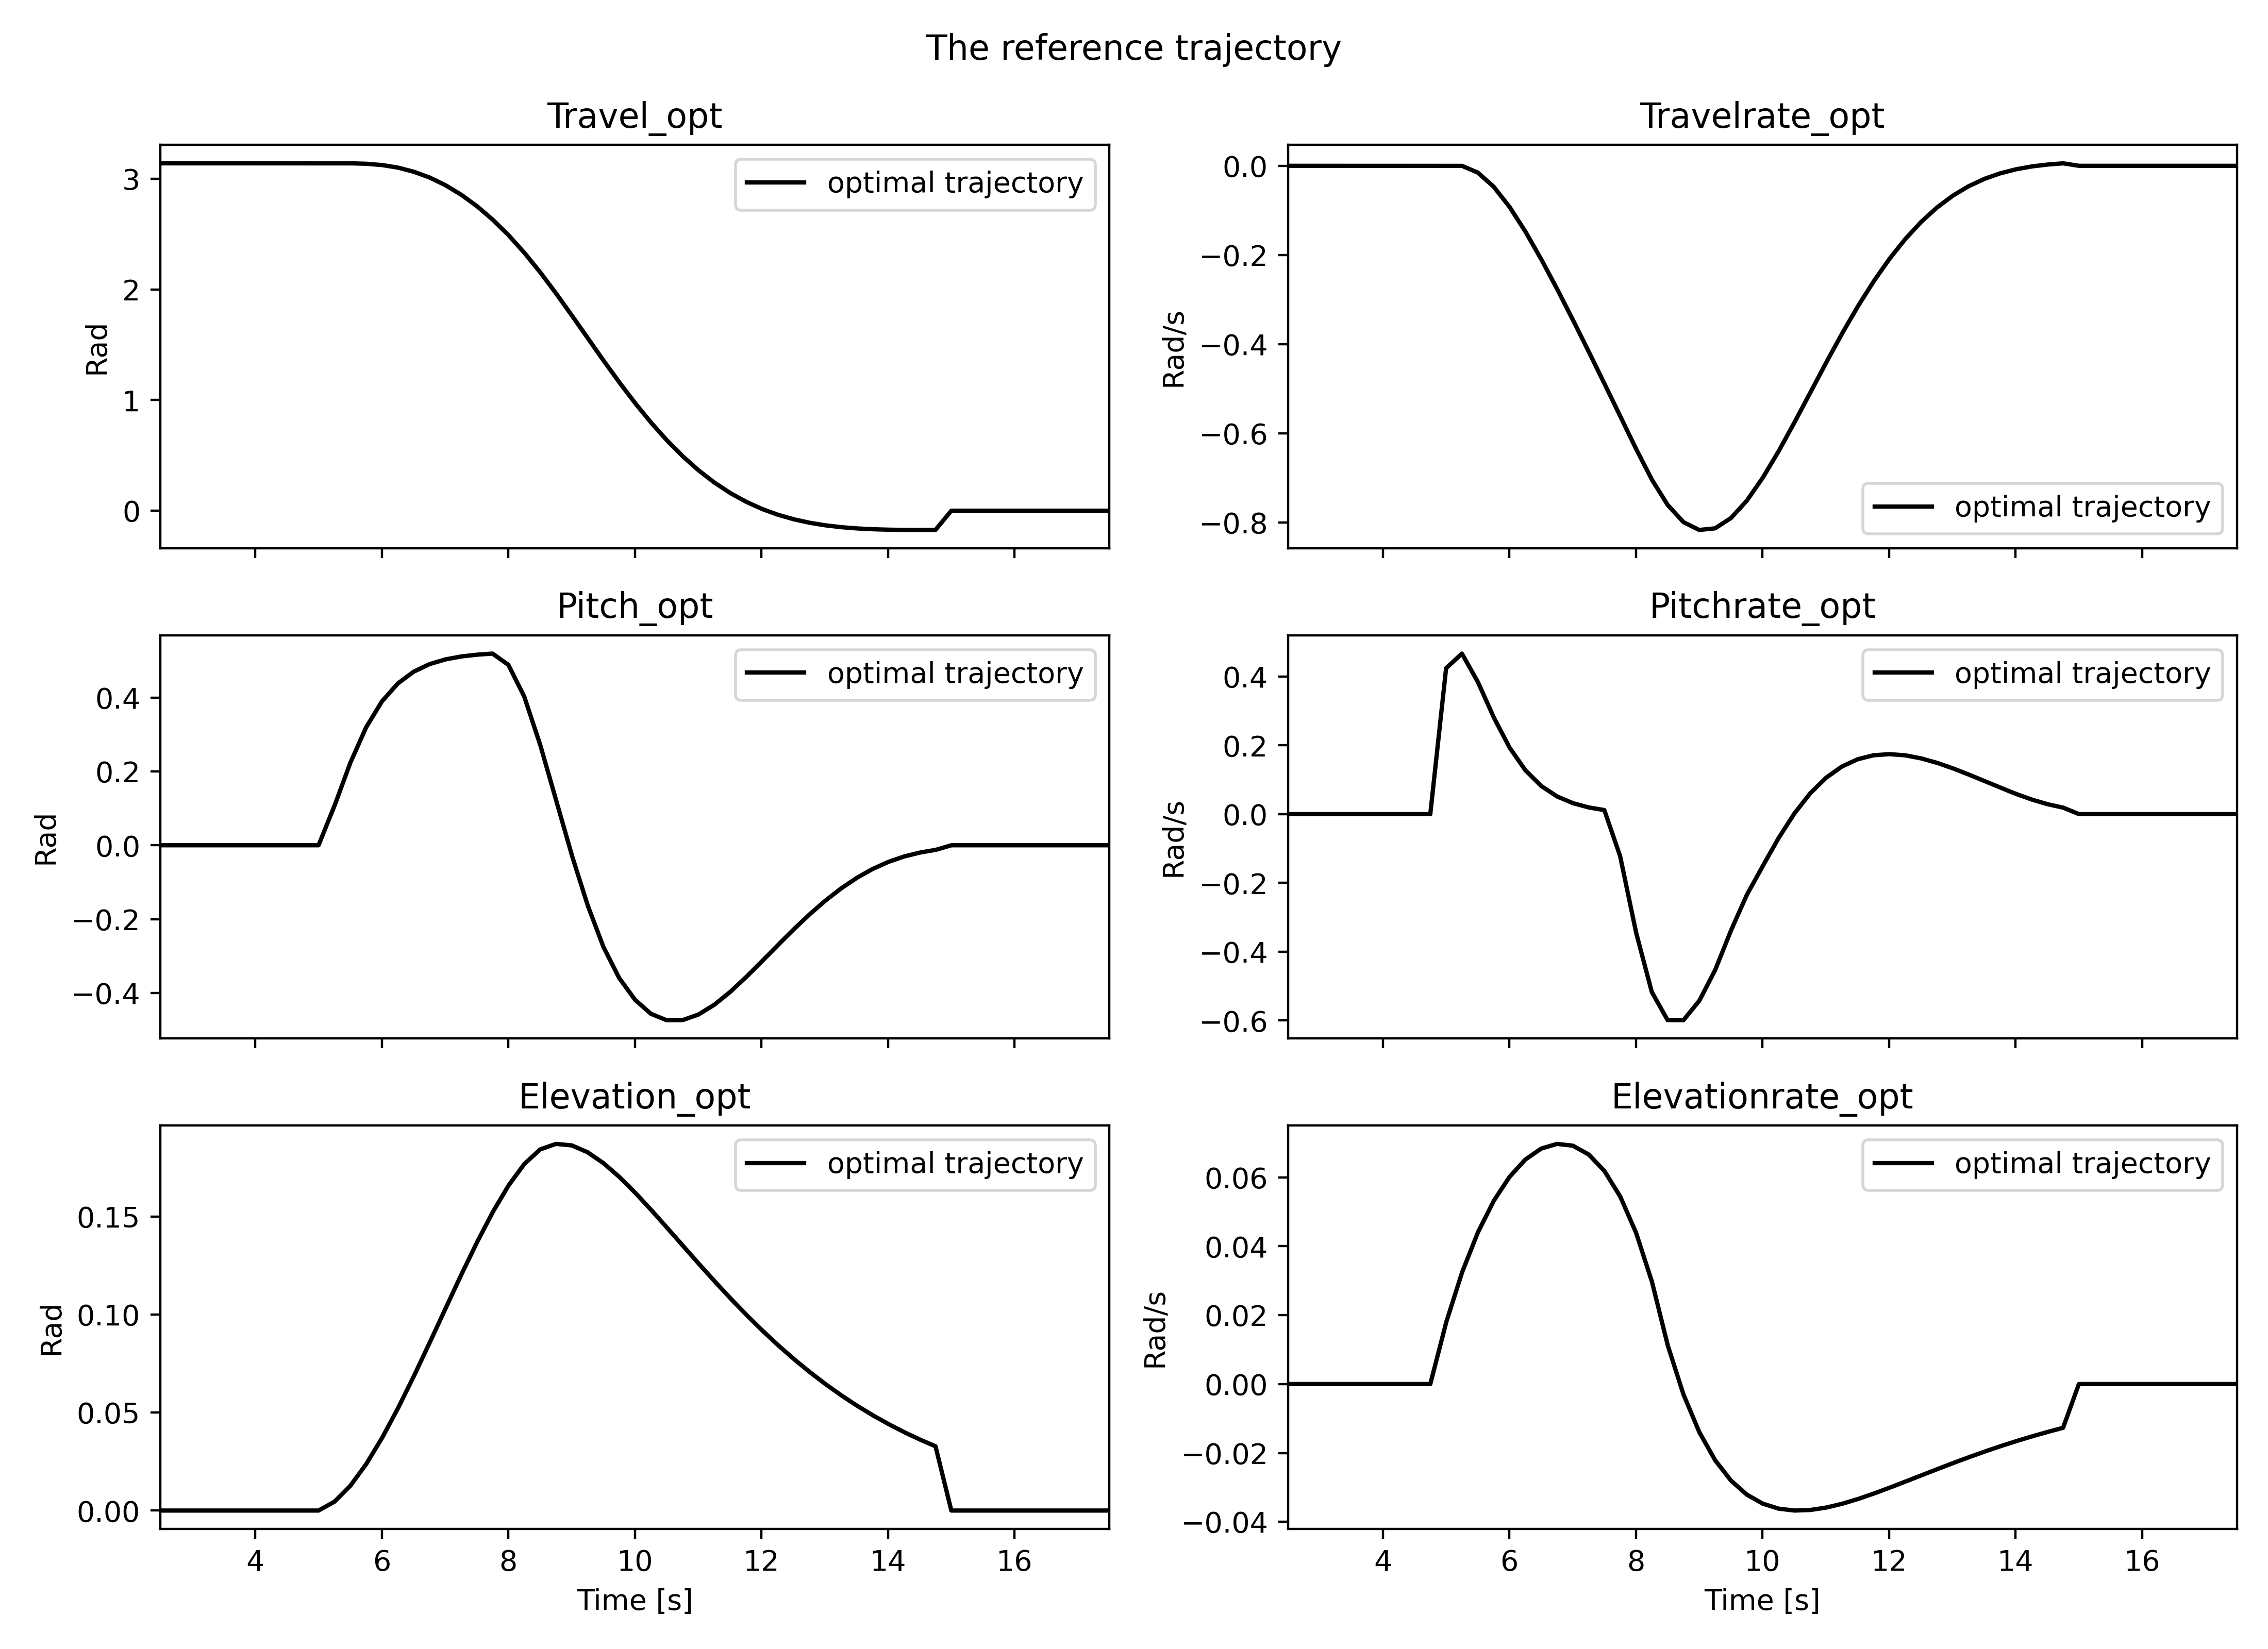
\includegraphics[width=\linewidth]{figures/LAB4_reference_trajectory.png}
	\caption{lol det ble visst plutselig 3x2 plots - fant en ish-fin workaround for å få det til å funke}
\end{figure}

In the tuning process we decided to keep R and Q as diagonal matrices. R was set constant equal the identity matrix, i.e. $R = I_2$. The diagonal elements of Q was then changed to get a good-tuned system. Each diagonal entry in Q corresponds to the corresponding stat in \cref{eq:lab4_cont_ss} \todo{REFORMULATE}, so the tuning process was done by tuning state-by-state. 

Since we are interested in following the optimal trajectory for the travel, we started by tuning this state, i.e. changing Q(1, 1) \todo{add ref to matlab script}. The figure below shows the helicopter states to the optimal trajectory for different Q(1, 1) values. As expected, a higher value of Q made the system use more \"fuel\" to follow the travel. Using too large value caused the helicopter's pitch to oscillate quite much, and too low resulted in a bad response.

\begin{figure}[h]
	\centering
	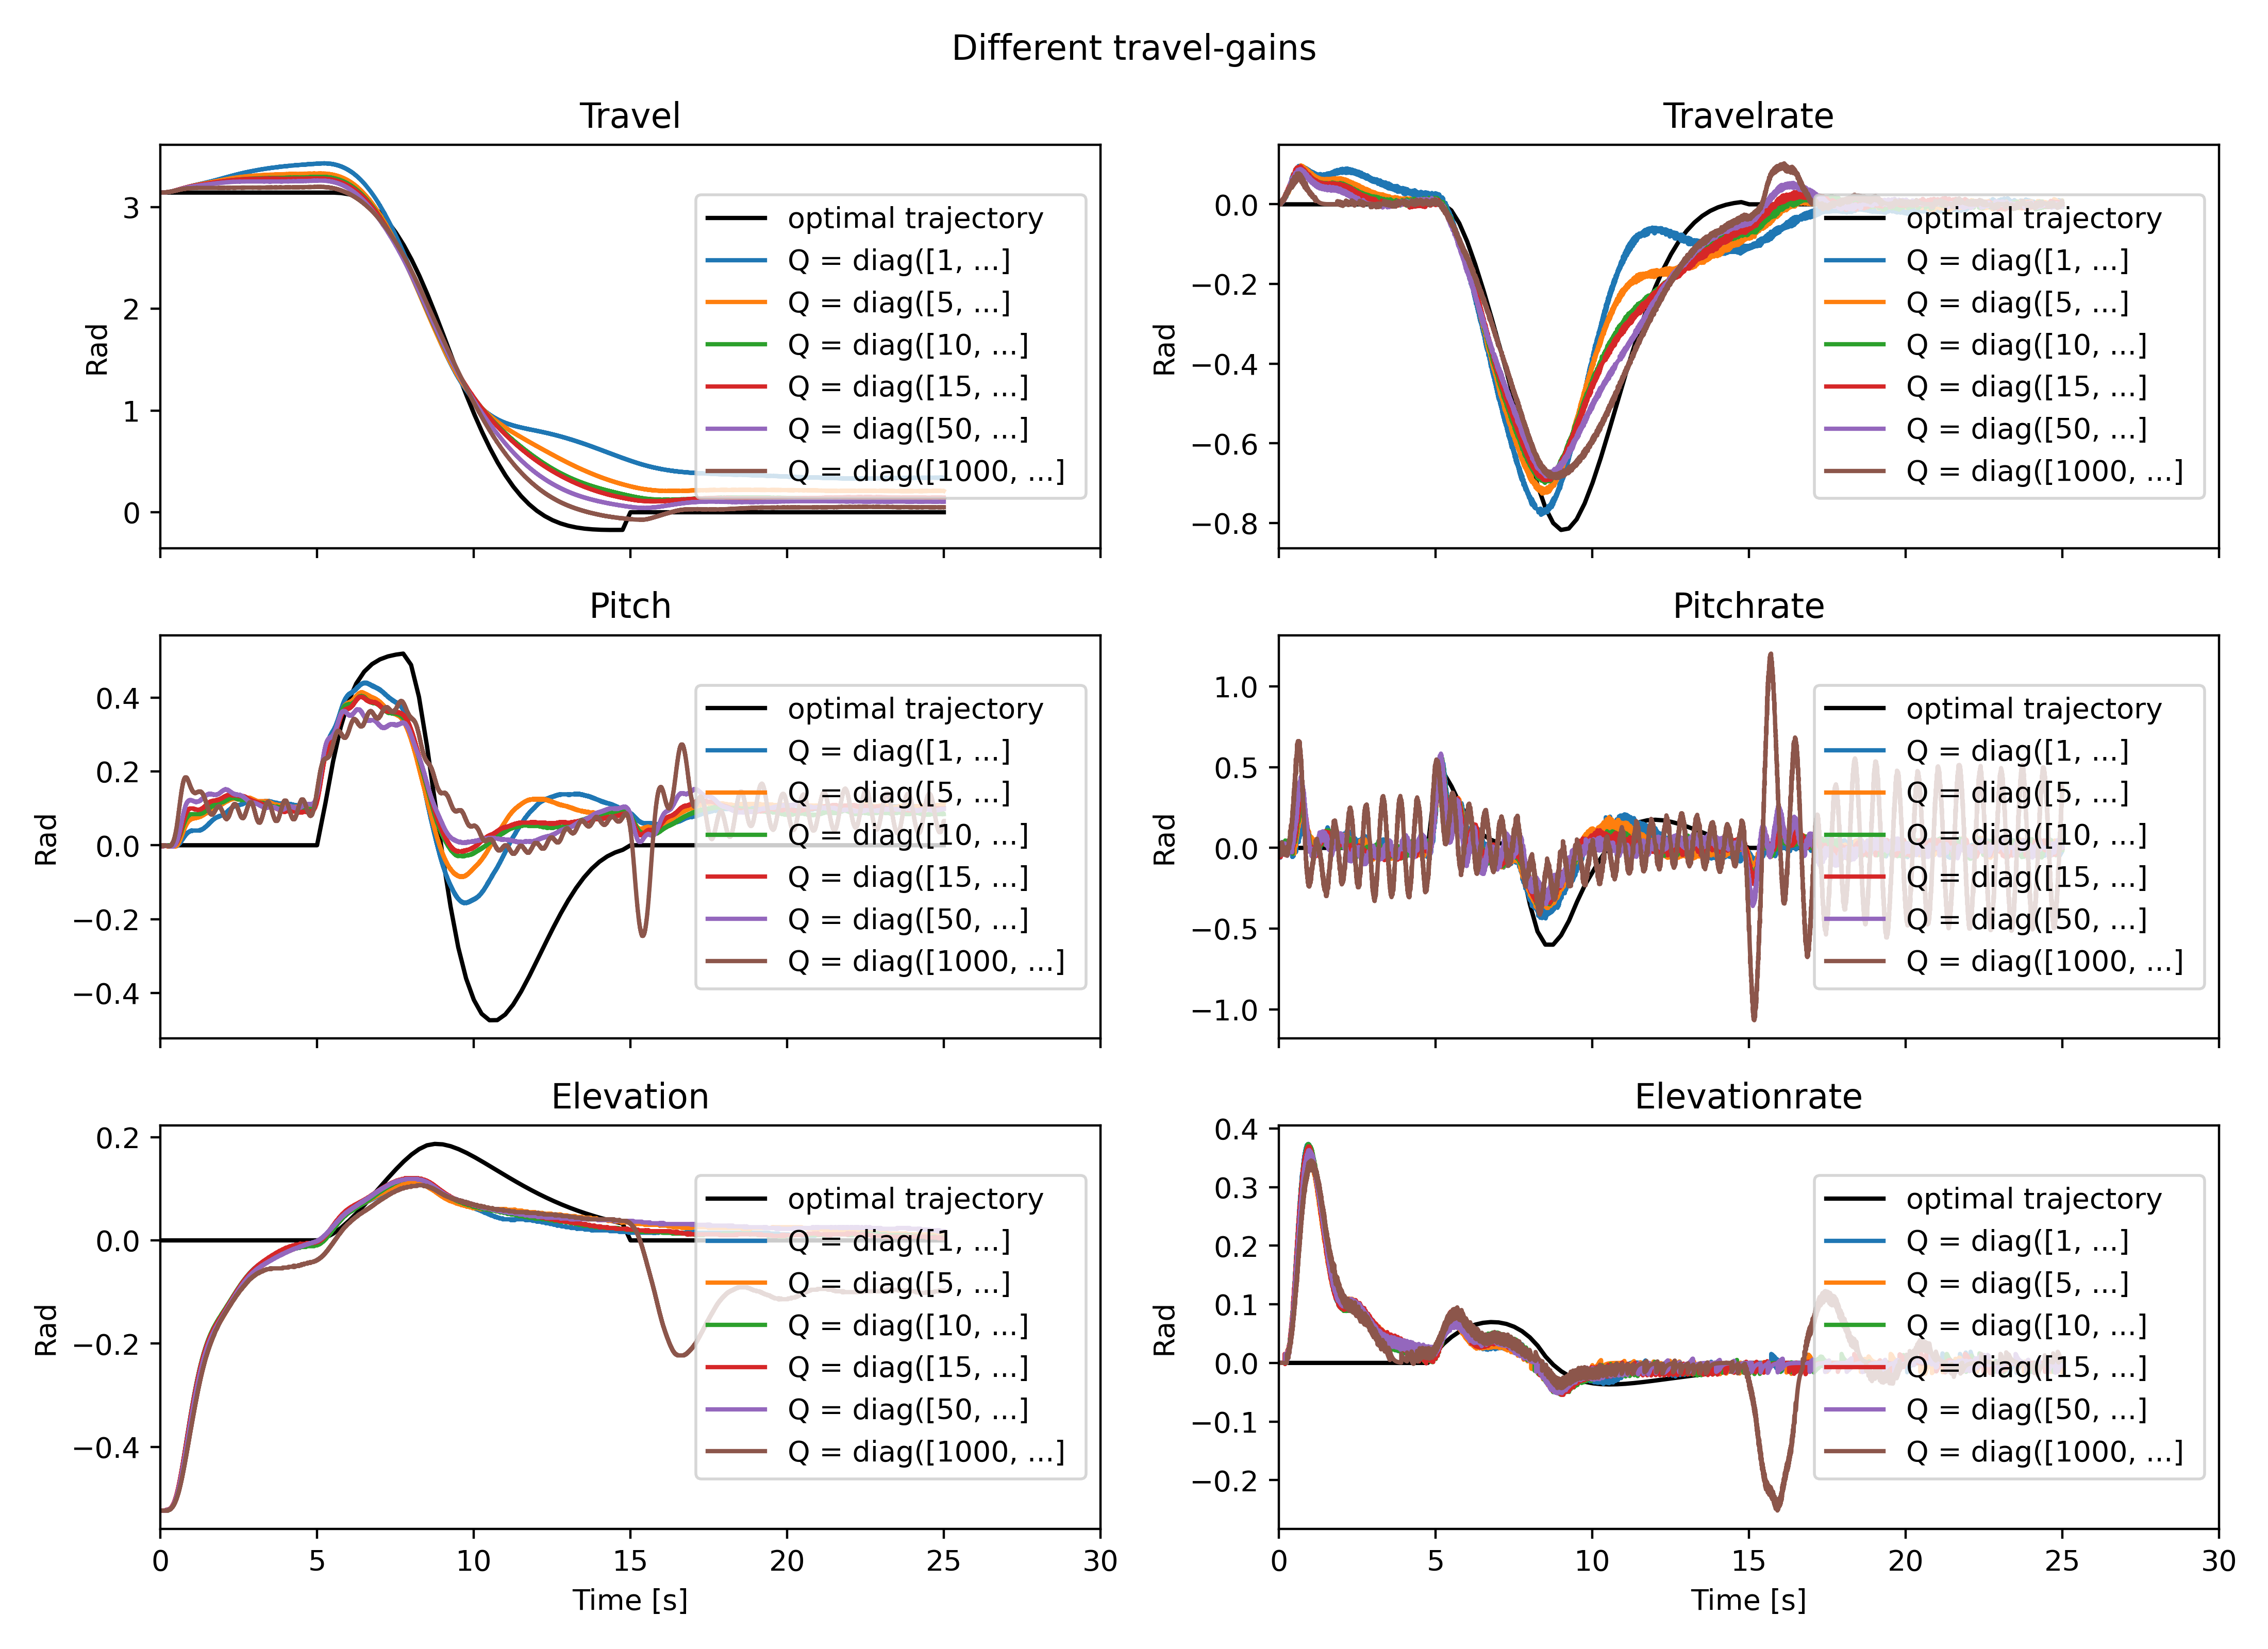
\includegraphics[width=\linewidth]{figures/LAB4_travel_gains.png}
	\caption{Her er alle verdiene vi brukte, bør nok rydde opp litt.}
\end{figure}

The group then proceeded to tuning the elevation. Since the helicopter did not have a good response for the elevation (SEE PLOT...) we decided to increase Q(5, 5) to use more \"fuel\" to get a response that followed the optimal elevation...
\missingfigure{Different Q(5, 5) values}


We also tried changing Q(3, 3) to see if we could get a better pitch response.
\missingfigure{Different Q(3, 3) values}

In the end we chose this configuration as out best tuning: 
\begin{equation}\label{key}
	\bm Q = \begin{bmatrix}
		0 & 0 & 0 & 0 & 0 \\
		0 & 0 & 0 & 0 & 0 \\
		0 & 0 & 0 & 0 & 0 \\
		0 & 0 & 0 & 0 & 0 \\
		0 & 0 & 0 & 0 & 0 \\
	\end{bmatrix}, 
	\bm R = \begin{bmatrix}
		1 & 0 \\ 
		0 & 1
	\end{bmatrix}
\end{equation}
%A signal generator was established to generate signals for the references $p_c$ and $e_c$. This signal generator is shown in \todo{Add ref}. The group chose to use a signal generator for tuning to guarantee a reference signal the helicopter was able to follow. The reason the optimal reference trajectory were not used in the tuning process, was that it was not certain this trajectory could be achieved by the helicopter. Therefore it seemed most reasonable to seperate tuning and optimal trajectory.

\subsection{Finding a reasonable trajectory}
With a good
 






\subsection{Decoupled model}
\textit{Answer 10.4.2.7}

\subsection{MATLAB and Simulink}
\textit{Code and diagrams go here}

\subsection{Optional exercise}
\textit{Which constraints did you add? What was the results? Plots? Discussion?}
\end{document}